\documentclass{scrreprt}
\usepackage{paralist}
\usepackage{graphicx}
\usepackage[final]{hcar}

\def\EMailRepl#1#2{\DoEMailRepl{#2} #1@\End}
\def\DoEMailRepl#1#2@#3\End
  {\if!#3!#2\else\DoDoEmailRepl{#1}{#2}#3\fi}
\def\DoDoEmailRepl#1#2#3@{#2#1#3}
\def\EAt{ @ }

%include polycode.fmt

\begin{document}

\begin{hcarentry}{Craftwerk}
\report{Malte Harder}
\status{Active Development}
\participants{Jannis Harder}% optional
\makeheader

Craftwerk is a 2D vector graphic library. The motivation was to have a graphic library that is able to generate output which can be embedded into {\LaTeX } as well as support for rendering with Cairo. Thus the library separates the graphic's data structure from any context dependency and the aim is to support various drivers. Currently a driver for output with the TikZ package (\url{http://sourceforge.net/projects/pgf/}) for {\LaTeX } is available. Using the additional { \verb craftwerk-cairo } and { \verb craftwerk-gtk } packages, direct rendering into PDF files or GTK widgets is possible. The { \verb craftwerk-gtk } package also provides functions to generate simple user interfaces for interactive graphics.

\begin{figure}[h]
  \centering
\begin{tabular}{cc}%{c c}
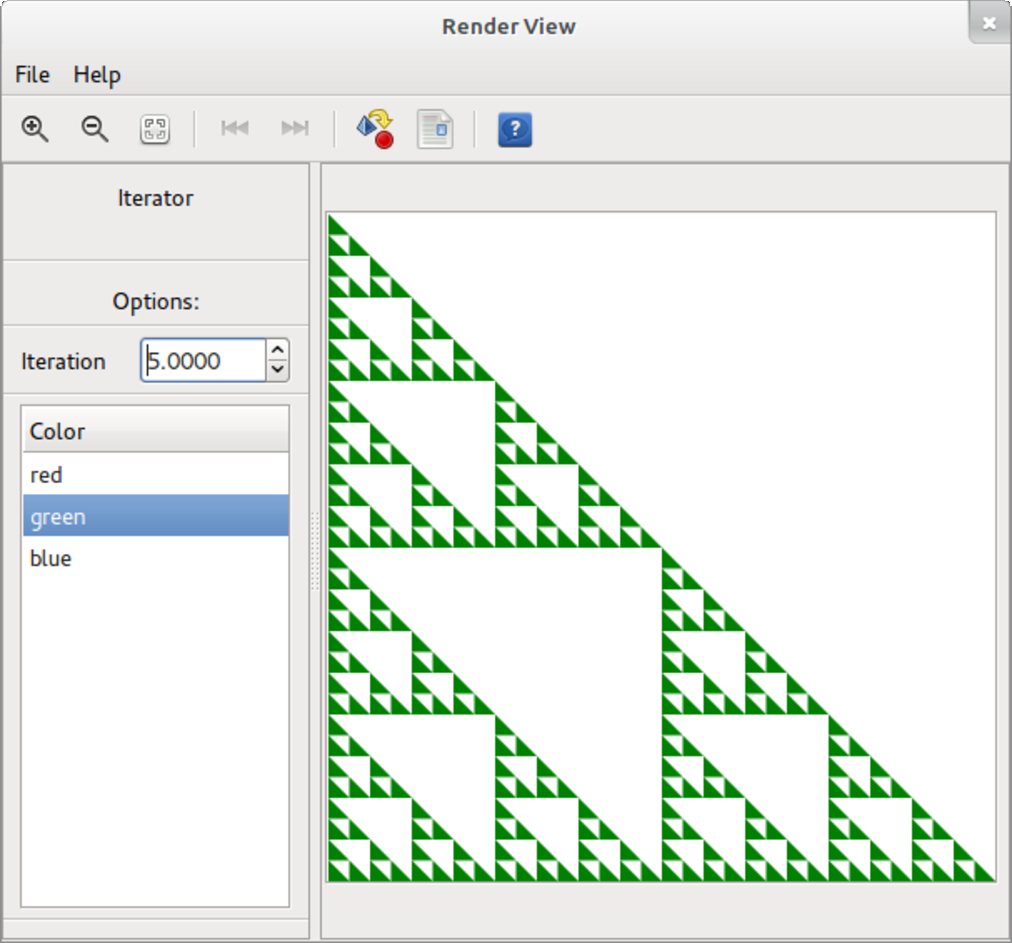
\includegraphics[width=6cm]{sierpinski}& 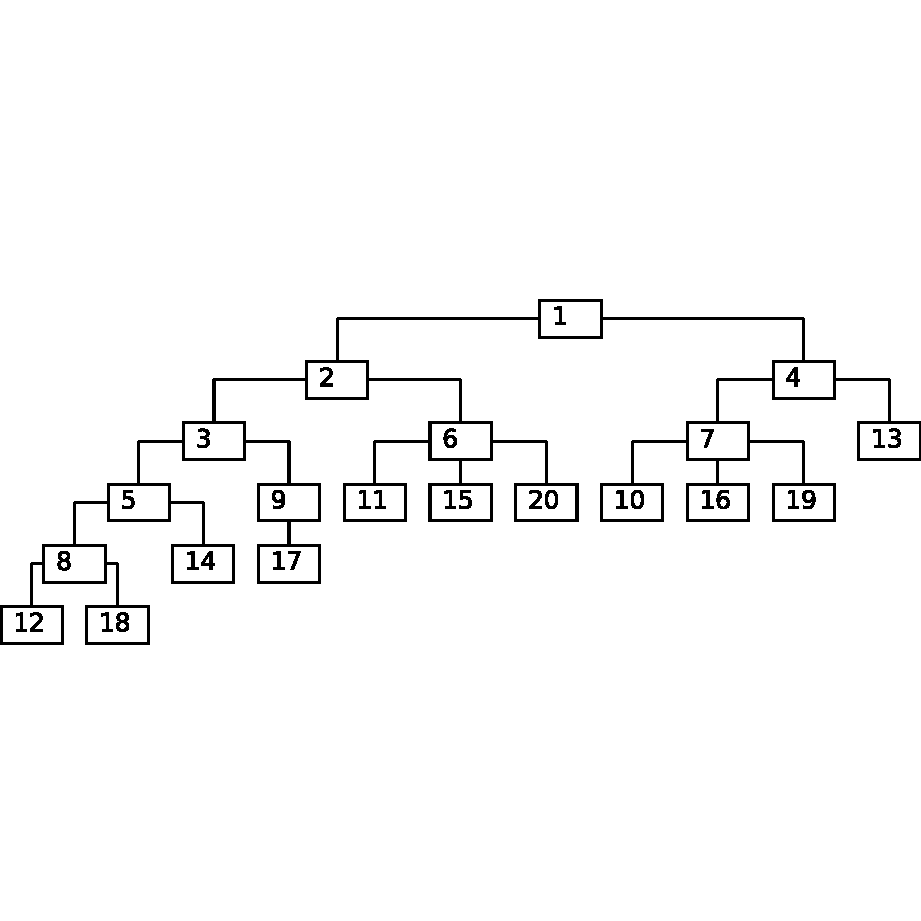
\includegraphics[width=6cm]{trees}\\
\end{tabular}
\end{figure}

The figure shows two examples, in the left image you can see a screenshot of the GTK interface for interactive graphics showing a Sierpi\'{n}ski triangle and the right image is a simple example of a tree rendered with the Cairo driver. Graphics or figures can be created in a hierarchical fashion including the application of styles and decorations to subnodes. The current functionality includes almost the complete Cairo function set extended by arrow tips and few primitives. The same function set is supported for TikZ output and graphics generated with the two drivers match closely. Immediate development tasks are:

\begin{itemize}
  \item Improvement of rendering speed in the Cairo driver.
  \item Better and unified text rendering capabilities.
  \item Refactoring of the UI module towards better usability.
\end{itemize}

Besides additional functionality, a long term goal is to support other drivers like Wumpus, Haha (ASCII rendering) or OpenGL. Craftwerk could also serve as an intermediate layer for libraries like { \verb plot } or {\verb chart } to enable {\LaTeX } export. At the moment the library is still at a preliminary stage and the next step is a consolidation of a basic feature set. Any contributions or ideas are welcome and the latest code as well as experiments with other drivers are available on GitHub. 

\FurtherReading
  \url{http://hackage.haskell.org/package/craftwerk-0.1}\\
  \url{http://mahrz.github.com/craftwerk}
\end{hcarentry}

\end{document}
